\documentclass[tcc,capa]{texufpel}

\usepackage[utf8]{inputenc} % acentuacao
\usepackage{graphicx} % para inserir figuras
\usepackage[T1]{fontenc}

\hypersetup{
    hidelinks, % Remove coloração e caixas
    unicode=true,   %Permite acentuação no bookmark
    linktoc=all %Habilita link no nome e página do sumário
}

\unidade{Centro de Desenvolvimento Tecnológico}
\curso{Ciência da Computação}
\nomecurso{Bacharelado em Ciência da Computação}
\titulocurso{Bacharel em Ciência da Computação}

\unidadeeng{Technology Development Center}
\cursoeng{Computer Science}


\title{Visual Sims: uma ferramenta que utiliza Computação Gráfica para auxiliar a aprendizagem}

\author{Sampaio}{Letícia}
\advisor[Prof.~Dr.]{Torchelsen}{Rafael Piccin}
% \coadvisor[Prof.~Dr.]{Aguiar}{Marilton Sanchotene de}
% \collaborator[Prof.~Dr.]{Aguiar}{Marilton Sanchotene de}

%Palavras-chave em PT_BR
\keyword{Computação Gráfica}
\keyword{WebGL}
\keyword{Simulação}
\keyword{Interatividade}

%Palavras-chave em EN_US
\keywordeng{Graphyc Computing}
\keywordeng{WebGL}
\keywordeng{Simulation}
\keywordeng{Interactivity}

\begin{document}

% \renewcommand{\advisorname}{Orientadora}           %descomente caso tenhas orientadora
%\renewcommand{\coadvisorname}{Coorientadora}      %descomente caso tenhas coorientadora

\maketitle 

\sloppy

\fichacatalografica

%\folhadeaprovacao

%Composição da Banca Examinadora
\begin{aprovacao}{18 de junho de 2021} %data da banca por extenso
\noindent Prof. Dr. Rafael Piccin Torchelsen (orientador)\\
Doutor em Ciência da Computação pela Universidade Federal do Rio Grande do Sul.\\[1cm]

\noindent Prof. Dr. Marilton Sanchotene de Aguiar\\
Doutor em Ciência da Computação pela Universidade Federal do Rio Grande do Sul.\\[1cm]

\noindent Profa. Dra. Tatiana Aires Tavares\\
Doutora em Engenharia Elétrica pela Universidade Federal do Rio Grande do Norte.\\[1cm]

\end{aprovacao}

%Opcional
\begin{dedicatoria}
  Dedico\ldots 
\end{dedicatoria}

%Opcional
\begin{agradecimentos}
  Agradeço\ldots 
\end{agradecimentos}

%Opcional
\begin{epigrafe}
  It's not stupid if it works.\\
  {\sc --- Sociedade}
\end{epigrafe}

%Resumo em Portugues (no maximo 500 palavras)
\begin{abstract}
Para alunos dos cursos de Ciência e Engenharia de Computação encontrar conteúdo para estudar é uma tarefa fácil, entretanto existem poucas fontes de pesquisa que disponibilizam um conteúdo interativo. Conceitos ensinados de forma apenas teórica podem surgir como barreira para uma parcela desses alunos, por isso transformar um conteúdo teórico em prático e tornar esse conteúdo acessível é o objetivo deste trabalho. Com isso, proponho um site com exemplos visuais e interativos de conteúdos abordados nas cadeiras de graduação dos cursos de Ciência e Engenharia de Computação. Utilizando conceitos de computação gráfica o aluno poderá visualizar exemplos e aprender de forma mais fácil o conteúdo abordado. Além da versão visual também será disponibilizado uma explicação textual do conteúdo. O site poderá dessa forma ser utilizado como ferramenta para estudo extra classe ou até como uma ferramenta para auxiliar o professor no ensino a distância.
\end{abstract}

%Resumo em Inglês (no maximo 500 palavras)
\begin{englishabstract}{Titulo do Trabalho em Ingles}
Bla blabla blablabla bla.  Bla blabla blablabla bla.  Bla blabla
blablabla bla.  Bla blabla blablabla bla.  Bla blabla blablabla bla.
Bla blabla blablabla bla.  Bla blabla blablabla bla.  Bla blabla
blablabla bla.  Bla blabla blablabla bla.  Bla blabla blablabla bla.
Bla blabla blablabla bla.  Bla blabla blablabla bla.  Bla blabla
blablabla bla.  Bla blabla blablabla bla.  Bla blabla blablabla bla.
Bla blabla blablabla bla.  Bla blabla blablabla bla.  Bla blabla
blablabla bla.  Bla blabla blablabla bla.  Bla blabla blablabla bla.
Bla blabla blablabla bla.
\end{englishabstract}

%Lista de Figuras
\listoffigures

%Lista de Tabelas
\listoftables

%lista de abreviaturas e siglas
\begin{listofabbrv}{ABNT}%coloque aqui a maior sigla para ajustar a distância
        \item[ABNT] Associação Brasileira de Normas Técnicas
        \item[V-Sync] Vertical Synchronization
        \item[WebGL] Web Graphics Library
        \item[OpenGL] Open Graphics Library
        \item[API] Application Programming Interface
        \item[HTML] HyperText Markup Language
        \item[CSS] Cascading Style Sheets
\end{listofabbrv}

%Sumario
\tableofcontents

\chapter{Introdução}



\chapter{Fundamentação teórica}

Neste capítulo são abordados temas pertinentes ao desenvolvimento de uma aplicação voltada ao ensino. 

\section{Simulação na educação}

Utilizar jogos ou simulações como ferramenta de aprendizado é uma tática que se aplica em diversas áreas do aprendizado. 

O uso de simulações para auxiliar o ensino é um tópico que pode ser aplicado em diversas áreas do aprendizado. 

Guiados por professores, os alunos de Ciência e Engenharia da Computação, têm o objetivo de aprender o conteúdo definido no programa da graduação, já a forma que o conhecimento é passado ao aluno fica por responsabilidade do professor. Para algumas cadeiras é muito difícil explicar a aplicação do conceito sendo passado, por ser um conceito abstrato ou por falta de recursos visuais. Nesses casos os professores podem recorrer a técnicas ou ferramentas que auxiliem os alunos a aprender de forma mais dinâmica o conteúdo.

Uma ferramenta que está muito presente no ensino extra classe é o Ambiente Virtual de Aprendizagem (AVA) que conforme Voss~\cite{Voss_Nunes_Herpich_Medina_2015} é um ambiente que aperfeiçoa a qualidade do ensino dos alunos, por meio de atividades além da sala de aula. Levando em consideração o contexto de ensino a distância, essas ferramentas se tornam essenciais para o desenvolvimento de um ensino de qualidade. 

No contexto computacional é comum aos professores buscarem formas de atrair a atenção dos alunos por meio de exemplos e atividades práticas que sejam interessantes para eles, como jogos e a robótica. Neste contexto simulações podem se tornar outro modo de cativar o interesse dos alunos, por serem aplicáveis para alunos de qualquer nível ou idade, além de retirar a dependência de um ambiente físico para exemplificação de um conteúdo~\cite{kincaid2003simulation}.

O conhecimento é fixado de forma diferente para cada pessoa, porém estímulos visuais se mostram mais eficientes no aprendizado, pois podem explorar de forma lúdica conceitos mais complexos~\cite{klawe1999computer}. Por este motivo o propósito do projeto proposto é fazer com que até as cadeiras que não possuem uma vertente prática possam utilizar de uma ferramenta dinâmica como auxiliar.

\section{Computação no Ensino}
\section{Outra seção}

\chapter{Trabalhos Relacionados}

Com base em simulações visuais e interativas os alunos podem explorar o que os conteúdos teóricos podem representar. Alguns trabalhos semelhantes já foram desenvolvidos e apresentaram resultado positivo em outros públicos alvo. Um trabalho similar, mas voltado aos alunos de ensino médio, é o site PHET~\cite{phet_2002}. Ele conta com diversas simulações que envolvem física, matemática e química. No site é possível acessar a biblioteca de simulações e interagir com variáveis e ver uma animação representando a mudança que essas variáveis trazem. 

Também temos o livro Immersive Linear Algebra~\cite{strom2017immersive} que conta com modelos em 3D e iterativos que ajudam na fixação e compreensão do conteúdo explicado. Com os modelos disponíveis no livro é possível ver as alterações que as fórmulas implicam nos gráficos e assim entender de forma gradual sua função.

Podemos utilizar o site WebGL Fundamentals~\cite{webgl_2017} também como referência de que contando com exemplos visuais o conteúdo sendo explicado se fixa melhor. No site aprendemos como utilizar a ferramenta WebGL, com exemplos iterativos junto à explicação.

\chapter{Desenvolvimento}

Este capítulo é dedicado ao desenvolvimento da plataforma Visual Sims e uma breve discussão acerca das decisões que foram tomadas para o seu desenvolvimento. Abordando desde o levantamento dos dados necessários quanto as tecnologias utilizadas, apresentando suas vantagens frente ao projeto proposto.

A etapa de desenvolvimento teve como resultado um site desenvolvido para web, direcionado ao uso em desktop. A busca por informação deve ser livre, portanto uma plataforma web tem o potencial de atingir a maior parte do publico alvo. Outra vantagem de uma aplicação web é sua capacidade de criação, a tela do computador podendo ser comparada com uma tela em branco, em que tudo pode ser criado.

\section{Escolha das tecnologias}

O desenvolvimento de páginas estáticas tradicionais, com HTML e CSS, possibilitam a criação de diversos sites com diferentes propósitos, com a utilização da API WebGL as possibilidades de criação aumentam ainda mais. A combinação de JavaScript com WebGL criam uma ferramenta adaptável ao usuário da web.

\subsection{WebGL}

WebGL é uma API em JavaScript que utiliza o elemento Canvas do HTML5 para renderização de elementos 2D e 3D. Esta API é uma evolução da API OpenGL, responsável por unificar 

Uma API é um conjunto de funções que tem como principal objetivo fazer a comunicação do software com o hardware. Dessa forma a API de WebGL além de fornecer funções que tornam a programação 2D e 3D mais prática, faz isso de uma forma mais otimizada, permitindo o acesso do navegador ao uso da GPU do computador. 

Para entendermos melhor em que momento o WebGL atua, precisamos entender o fluxo de criação de um objeto em uma cena. Este processo é composto de diversas etapas, e muitas delas não necessitam de alterações. Na figura~\ref{pipeline_grafico} podemos ver o pipeline de redenrização.

\begin{figure}[htbp]
  \centering 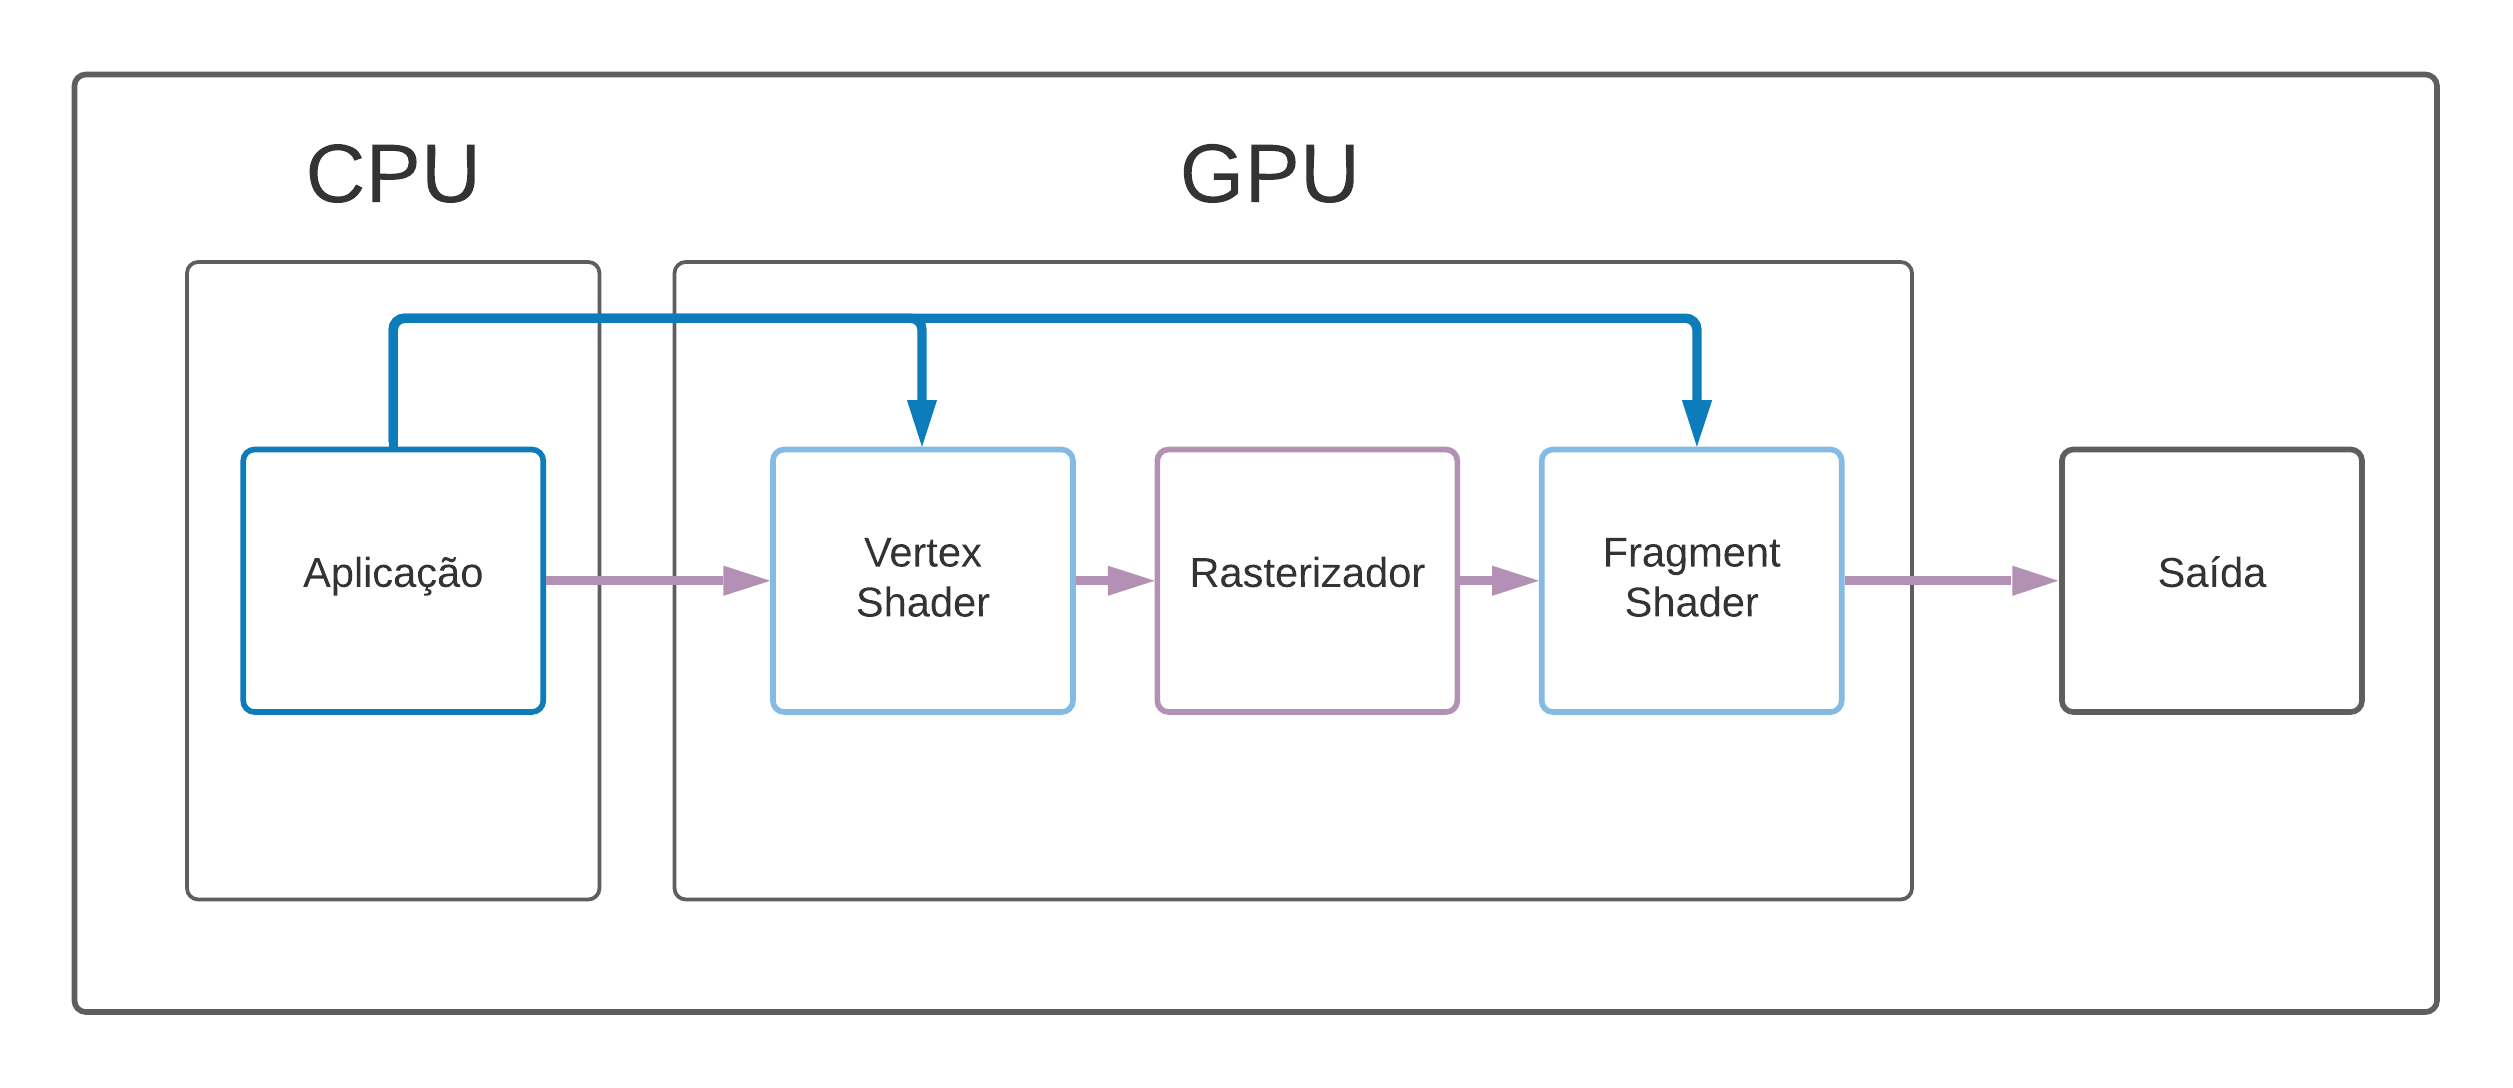
\includegraphics[scale=.7]{pipeline_grafico}
  \caption{Pipeline Gráfico}
  \label{pipeline_grafico}
\end{figure}% todo melhorar a imagem, colocar as outras etapas

Começando o processo de renderização a primeira etapa passar pelo Vertex Shader, ele é responsável por receber um conjunto de vértices definidos na aplicação e enviar para o rasterizador estes vértices mapeados. O Rasterizador por sua vez tem o papel de transformar os vértices em pixels, para que assim o Fragment Shader possa colorir eles.

Na figura podemos observar destacado em azul as etapas que são programáveis. São elas que recebem o suporte do WebGL. As setas em roxo representam o fluxo de dados durante a execução do programa. 

Portanto, o WebGL fornece suporte para a criação do Vertex Shader, com a utilização da linguagem JavaScript, e o Fragment Shader, utilizando a linguagem GLSL. 

\subsection{React}

React é uma das bibliotecas para JavaScript mais utilizadas na criação de novos projetos web da atualidade. A sua popularidade se dá pela sua estrutura e reusabilidade. Dentro do React é possível criar estruturas modulares que serão reaproveitadas em diversas partes do projeto. 

\subsection{Three.js}

Three.js é uma biblioteca que abstrai algumas declarações que precisariamos fazer utilizando somente JavaScript e GLSL para programação em WebGL. 

\subsection{React Three Fiber}

React Three Fiber é a biblioteca que facilita a programação utilizando Three.js e React. Ela permite a criação de componentes 3D reutilizáveis dentro da aplicação.

\section{Coleta de dados}

Para o desenvolvimento da plataforma Visual Sims foi necessária uma coleta de dados acerca das simulações que seriam apresentadas como exemplo. O modelo de simulação desenvolvido foi sobre o recurso V-Sync, conceito que não consta no currículo dos cursos de computação, mas possibilita um melhor entendimento sobre o conceito de frames por segundo. Além de ter uma visão de renderização além de apenas um quadro.

A seguir irei aprofundar os conhecimentos sobre o recurso e falar sobre a vantagem de apresentar como conteúdo extra.

\subsection{V-Sync}

O V-Sync (Vertical Synchronization) é uma funcionalidade disponível em algumas placas de vídeo para sincronização de quadros do computador com a tela. Embora nossas tecnologias sejam versáteis podemos enfrentar problemas ao alinhar a quantidade de quadros enviadas pelo computador com a quantidade de quadros que a tela aceita.

Essa diferença se torna um problema quando é possível ver uma quebra no quadro. Essa quebra ocorre porque a velocidade de renderização do quadro atual é diferente da velocidade em que os quadros estão chegando.Sendo a renderização ser feita de cima para baixo, enquanto um quadro está terminando de renderizar o próximo já inicia o processo, por isso acaba parecendo um corte na tela horizontalmente.



\section{Criação do Projeto}


\chapter{Resultados e Discussões}



\section{Formulário teste}

\chapter{Conclusão}

Como trabalhos futuros temos 

\bibliographystyle{abnt}
\bibliography{bibliografia} 

% Apêndices (Opcional) - Material produzido pelo autor
% \apendices
% \chapter{Um Apêndice}

% Anexos (Opcional) - Material produzido por outro
% \anexos
% \chapter{Um Anexo}

% \chapter{Outro Anexo}

% Faz a capa do CDROM
% \makecover

\end{document}

